%
% File: chapters/appendices/app0A.tex
% Appendices A--E
%
\chapter{C4 Diagrams}
\label{app:c4}
\setlength{\parskip}{1em}

This appendix reproduces the three-level C4 model~\cite{brownc42018} that frames the system architecture. The Mermaid sources are maintained alongside the running code in \texttt{docs/architecture/c4-system-context.md}, \texttt{c4-containers.md}, and \texttt{c4-components-planning.md}; the rendered images are placed under \texttt{figures/c4/} as PNG exports to keep the thesis self-contained.

Figure~\ref{fig:c4-context} is the Level~1 system context: who interacts with the platform, and which external systems the platform depends on. Figure~\ref{fig:c4-containers} is the Level~2 container view, showing the deployable units (mobile app, web landing, Django web, two Celery containers, RDS, ElastiCache, S3, the ETL pipeline, and the external SaaS services). Figure~\ref{fig:c4-planning} zooms into the planning service in Level~3, exposing the call chain from the REST handler through the orchestrator, candidate pool, scorer (deterministic and LightGBM-augmented), CP-SAT, and the post-processing steps that materialise the shopping list and push notification.

\begin{figure}[H]
\centering
\IfFileExists{figures/c4/c4-context.png}{%
  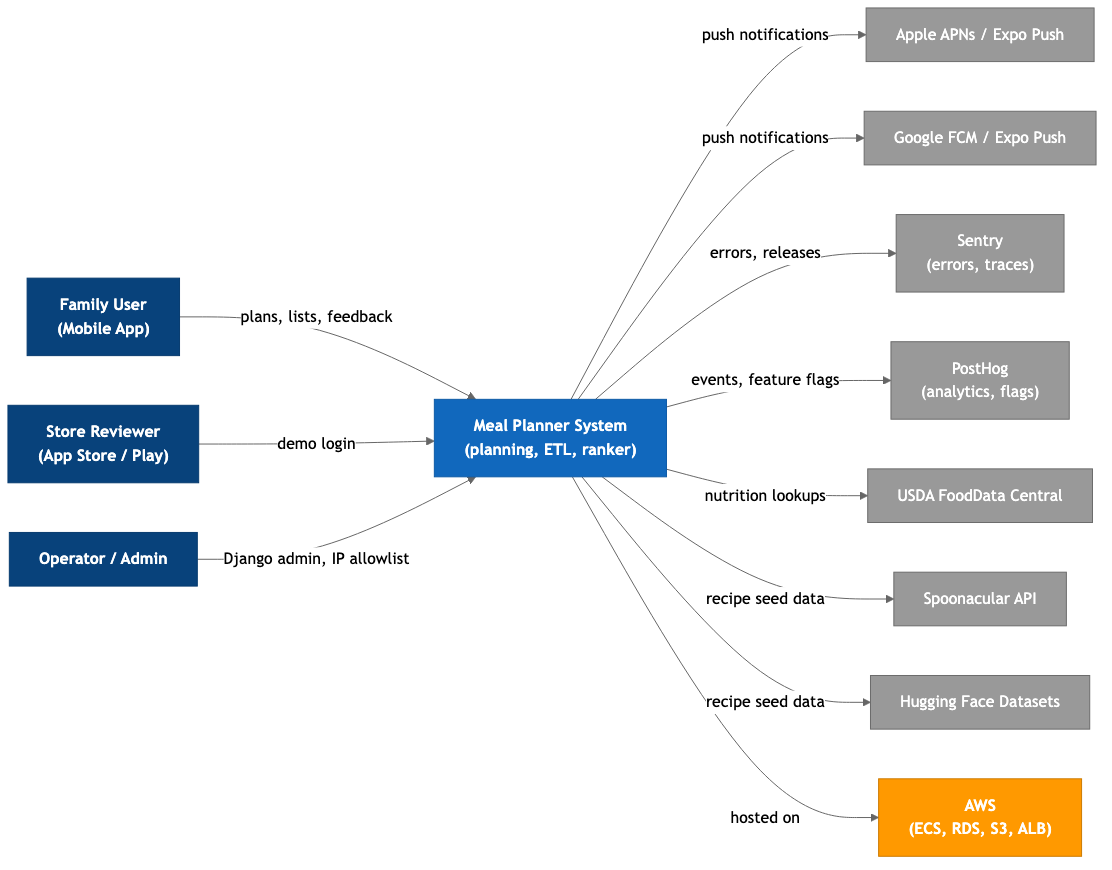
\includegraphics[width=0.95\textwidth]{figures/c4/c4-context.png}%
}{%
  \fbox{\parbox[c][6cm][c]{0.9\textwidth}{\centering Placeholder: \texttt{figures/c4/c4-context.png}}}%
}
\caption{C4 Level~1 --- System context.}
\label{fig:c4-context}
\end{figure}

\begin{figure}[H]
\centering
\IfFileExists{figures/c4/c4-container.png}{%
  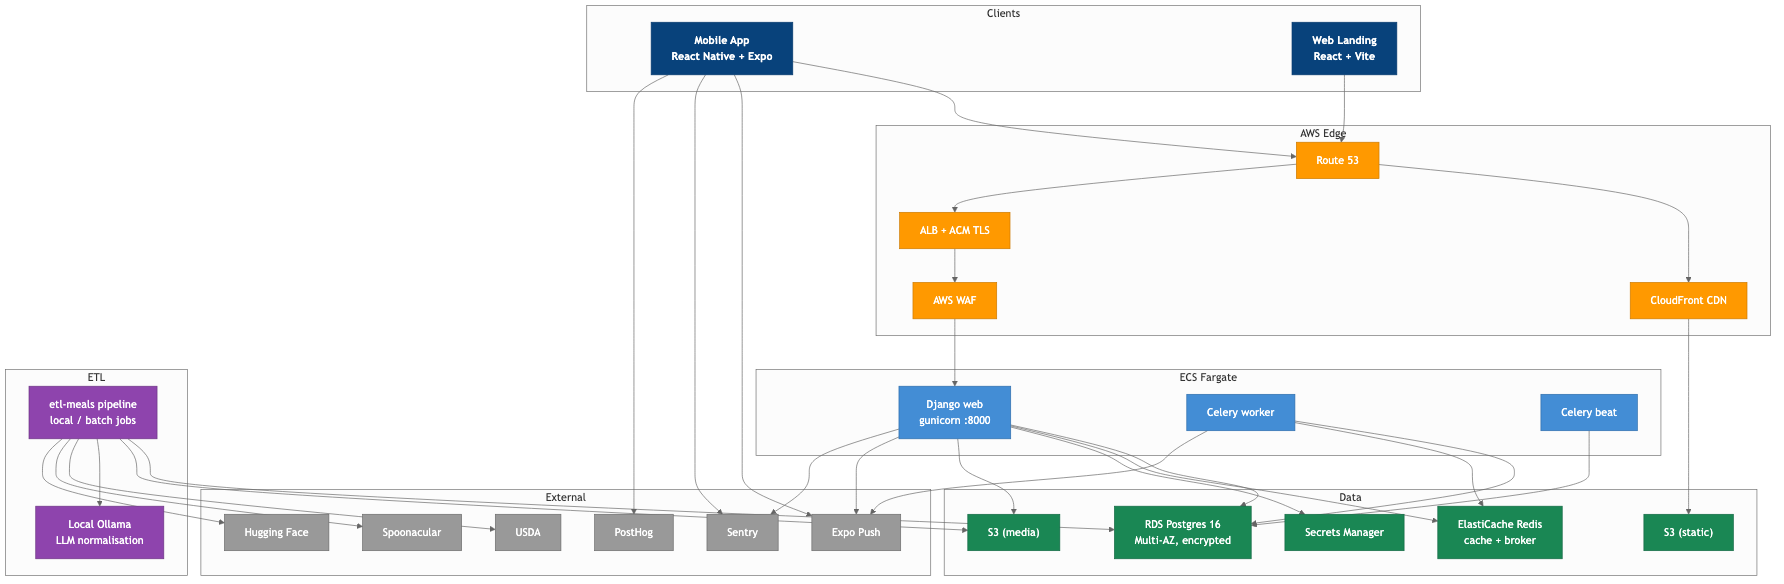
\includegraphics[width=0.95\textwidth]{figures/c4/c4-container.png}%
}{%
  \fbox{\parbox[c][6cm][c]{0.9\textwidth}{\centering Placeholder: \texttt{figures/c4/c4-container.png}}}%
}
\caption{C4 Level~2 --- Containers.}
\label{fig:c4-containers}
\end{figure}

\begin{figure}[H]
\centering
\IfFileExists{figures/c4/c4-component-planning.png}{%
  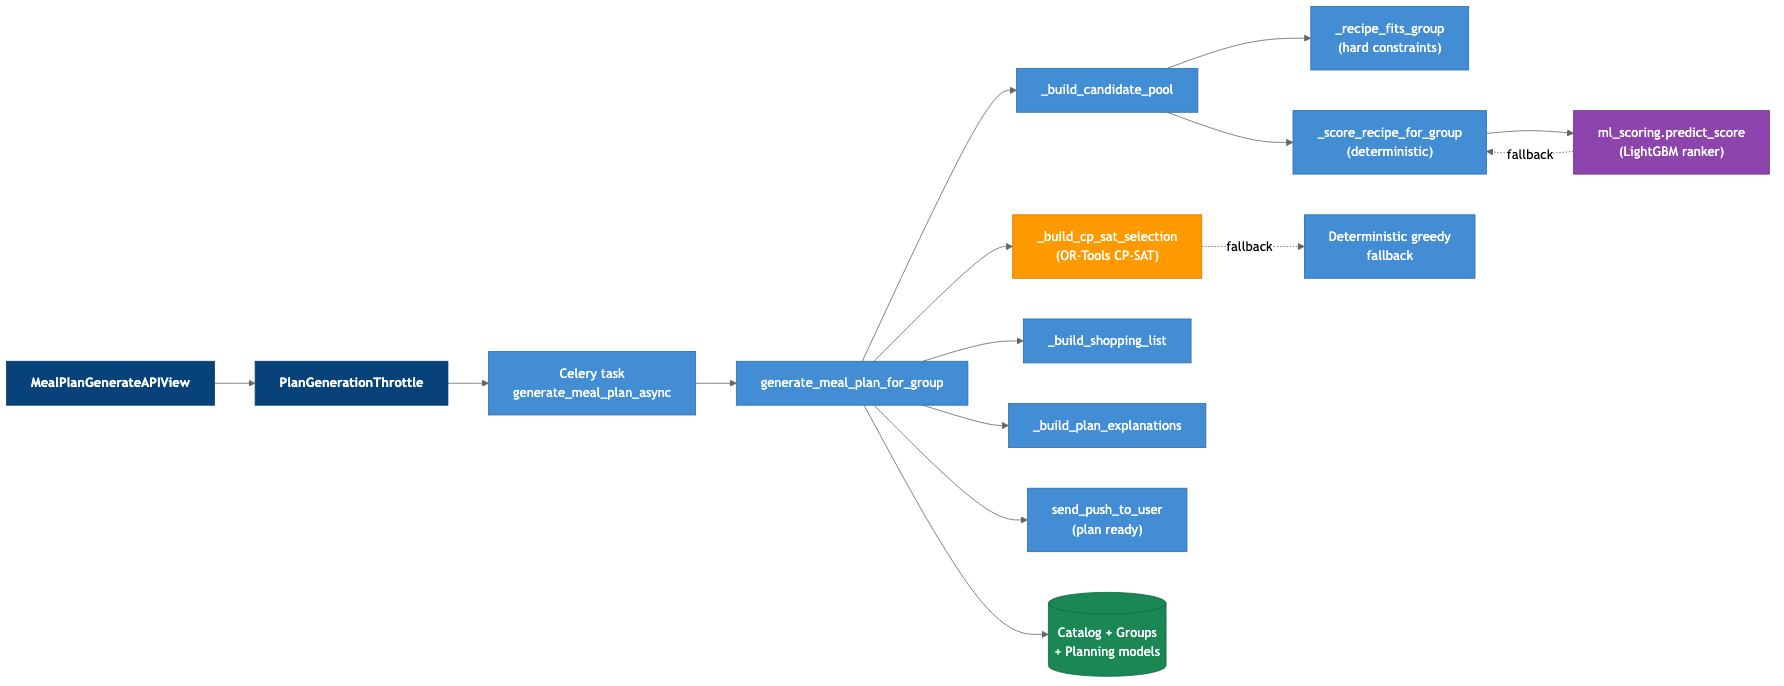
\includegraphics[width=0.95\textwidth]{figures/c4/c4-component-planning.png}%
}{%
  \fbox{\parbox[c][6cm][c]{0.9\textwidth}{\centering Placeholder: \texttt{figures/c4/c4-component-planning.png}}}%
}
\caption{C4 Level~3 --- Planning service components.}
\label{fig:c4-planning}
\end{figure}

\clearpage


\chapter{Entity Relationship Overview}
\label{app:er}

Table~\ref{tab:entities-full} enumerates the persisted domain entities and their owner apps. The diagram in Figure~\ref{fig:er} visualises the most important relationships using Mermaid \texttt{erDiagram} notation. The Mermaid source lives under \texttt{docs/diploma/diagrams/er-overview.mmd}, and the figure is rendered with \texttt{mmdc} (Mermaid CLI). For an exhaustive auto-generated dump including every column, the alternative \texttt{python manage.py graph\_models -a -o schema.png} (provided by the \texttt{django-extensions} package) can be used.

\begin{longtable}{|l|l|p{8cm}|}
\caption{Persisted domain entities by Django app.}
\label{tab:entities-full}\\
\hline
App & Entity & Purpose \\
\hline
\endfirsthead
\hline
App & Entity & Purpose \\
\hline
\endhead
users    & User                  & Authentication principal (email-as-login) \\
users    & UserSettings          & Notifications, measurement system, currency \\
groups   & Group                 & Household with budget, region, planning defaults \\
groups   & GroupMember           & Member with goal and macro targets \\
groups   & MemberConstraint      & Allergies, religious bans, dislikes \\
groups   & GroupPreference       & Cooking time, repeat tolerance, scalar weights \\
catalog  & Tag                   & Recipe tag with key and label \\
catalog  & Ingredient            & Canonical ingredient \\
catalog  & IngredientPrice       & Regional price reference \\
catalog  & IngredientSubstitution& Substitution candidates with reason \\
catalog  & Recipe                & Recipe with quality score and metadata \\
catalog  & RecipeTag             & Recipe-to-tag link \\
catalog  & RecipeStep            & Recipe instruction step \\
catalog  & RecipeIngredient      & Recipe-to-ingredient link with quantity and unit \\
catalog  & RecipeNutrition       & Per-serving and total macros \\
catalog  & FavoriteRecipe        & User favourite \\
catalog  & RecipeVersion         & Snapshot for audit \\
planning & MealPlan              & Plan with horizon, scores, optimiser metadata \\
planning & MealPlanDay           & Daily bucket \\
planning & MealPlanItem          & Recipe assigned to a (day, meal) slot \\
planning & MealItemAdaptation    & Per-member adaptation suggestion \\
planning & ShoppingList          & Aggregated procurement artifact \\
planning & ShoppingListItem      & Single shopping line \\
planning & PlanExplanation       & Human-readable plan rationale \\
planning & PlanGenerationRun     & Asynchronous run record \\
planning & PantryItem            & Pantry item with optional expiry \\
planning & ShareLink             & Read-only public link \\
feedback & RecipeFeedback        & Like, dislike, or rating with reason \\
feedback & PlanFeedback          & Multi-axis satisfaction \\
feedback & InteractionEvent      & Generic auditable interaction \\
feedback & Notification          & In-app notification \\
devices  & Device                & Expo push token with platform metadata \\
\hline
\end{longtable}

\begin{figure}[H]
\centering
\IfFileExists{figures/er/er-overview.png}{%
  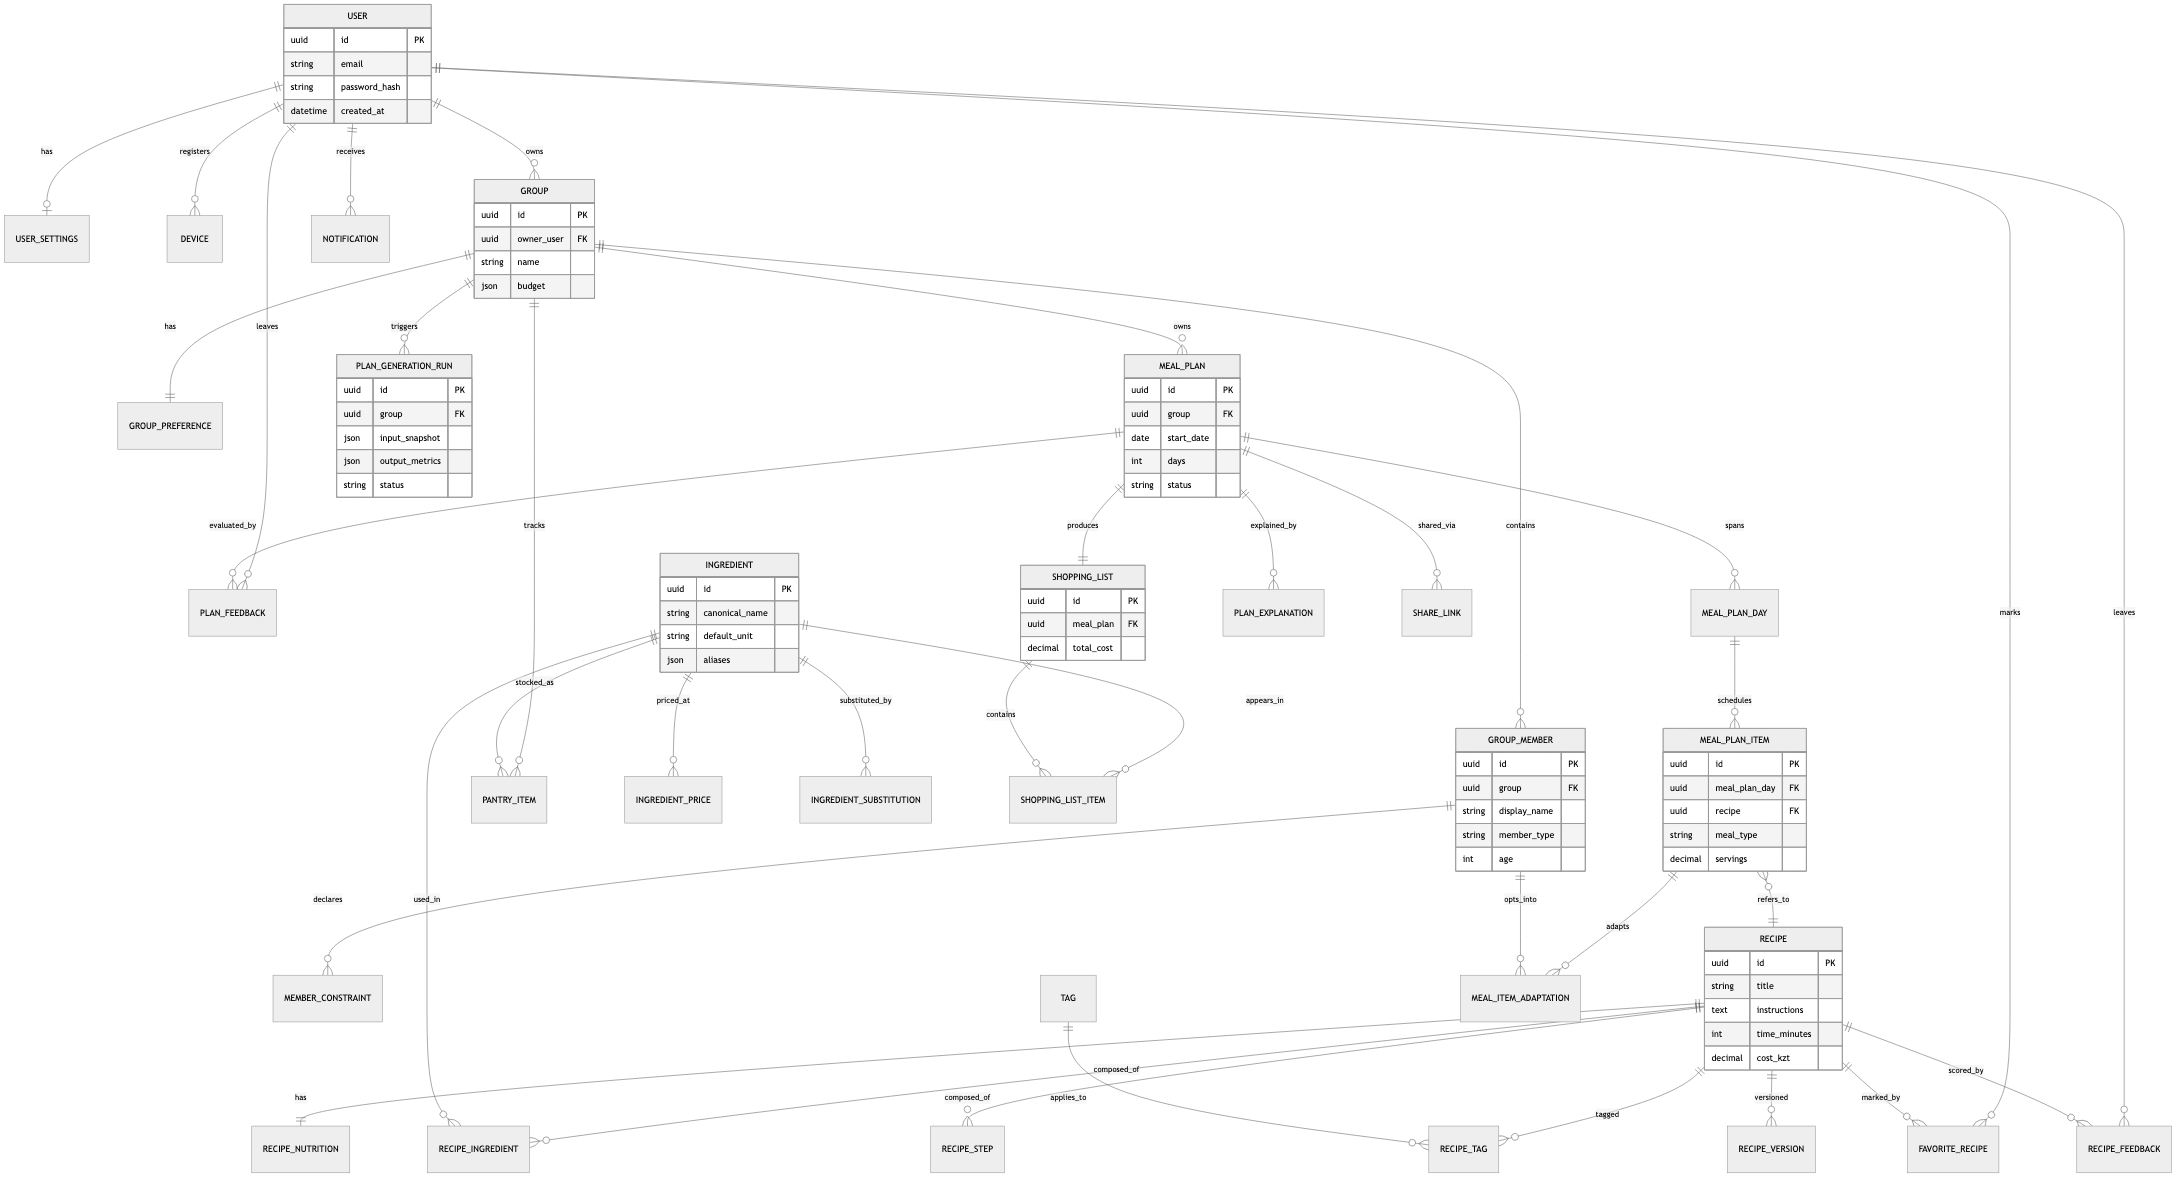
\includegraphics[width=\textwidth,height=0.85\textheight,keepaspectratio]{figures/er/er-overview.png}%
}{%
  \fbox{\parbox[c][6cm][c]{0.9\textwidth}{\centering Placeholder: \texttt{figures/er/er-overview.png}}}%
}
\caption{Domain ER overview across users, groups, catalog, planning, feedback, and devices apps. Audit-only and link tables (RecipeVersion, ShareLink, InteractionEvent, Notification, Device) are omitted for visual clarity.}
\label{fig:er}
\end{figure}

\clearpage


\chapter{API Surface Map}
\label{app:api}

The public API is versioned under \texttt{/api/v1/}. Endpoints are grouped by business function.

\paragraph{Authentication and account.}
\begin{itemize}
\item \texttt{/api/v1/auth/sign-up} (POST)
\item \texttt{/api/v1/auth/log-in} (POST)
\item \texttt{/api/v1/auth/log-out} (POST)
\item \texttt{/api/v1/auth/refresh} (POST)
\item \texttt{/api/v1/auth/me} (GET)
\item \texttt{/api/v1/auth/profile} (GET, PATCH)
\item \texttt{/api/v1/auth/account/delete} (POST)
\item \texttt{/api/v1/auth/account/export} (GET)
\item \texttt{/api/v1/profile} (GET, PATCH) --- product profile
\item \texttt{/api/v1/settings} (GET, PATCH)
\end{itemize}

\paragraph{Groups, members, constraints, preferences.}
\begin{itemize}
\item \texttt{/api/v1/groups} (GET, POST)
\item \texttt{/api/v1/groups/active} (GET)
\item \texttt{/api/v1/groups/\{group\_id\}} (GET, PATCH)
\item \texttt{/api/v1/groups/\{group\_id\}/activate} (POST)
\item \texttt{/api/v1/groups/\{group\_id\}/members} (GET, POST)
\item \texttt{/api/v1/groups/\{group\_id\}/preferences} (GET, PATCH)
\item \texttt{/api/v1/groups/\{group\_id\}/setup-summary} (GET)
\item \texttt{/api/v1/groups/\{group\_id\}/dashboard} (GET)
\item \texttt{/api/v1/members/\{member\_id\}} (GET, PATCH, DELETE)
\item \texttt{/api/v1/members/\{member\_id\}/constraints} (GET, POST)
\item \texttt{/api/v1/constraints/\{constraint\_id\}} (PATCH, DELETE)
\end{itemize}

\paragraph{Catalog, favourites, ingredients.}
\begin{itemize}
\item \texttt{/api/v1/recipes} (GET)
\item \texttt{/api/v1/recipes/tags} (GET)
\item \texttt{/api/v1/recipes/categories} (GET)
\item \texttt{/api/v1/recipes/search-suggestions} (GET)
\item \texttt{/api/v1/recipes/\{recipe\_id\}} (GET)
\item \texttt{/api/v1/favorites/recipes} (GET, POST)
\item \texttt{/api/v1/favorites/recipes/\{recipe\_id\}} (DELETE)
\item \texttt{/api/v1/ingredients} (GET)
\item \texttt{/api/v1/ingredients/\{ingredient\_id\}/prices} (GET)
\end{itemize}

\paragraph{Planning, runs, lifecycle.}
\begin{itemize}
\item \texttt{/api/v1/groups/\{group\_id\}/meal-plans} (GET)
\item \texttt{/api/v1/groups/\{group\_id\}/meal-plans/generate} (POST)
\item \texttt{/api/v1/groups/\{group\_id\}/meal-plans/current} (GET)
\item \texttt{/api/v1/meal-plans/\{meal\_plan\_id\}} (GET)
\item \texttt{/api/v1/meal-plans/\{meal\_plan\_id\}/days/\{day\_index\}} (GET)
\item \texttt{/api/v1/meal-plan-items/\{item\_id\}/replace} (POST)
\item \texttt{/api/v1/meal-plan-items/\{item\_id\}/adaptations} (GET, POST)
\item \texttt{/api/v1/meal-plan-items/\{item\_id\}/adaptations/\{adaptation\_id\}} (PATCH, DELETE)
\item \texttt{/api/v1/meal-plans/\{meal\_plan\_id\}/shopping-list} (GET)
\item \texttt{/api/v1/meal-plans/\{meal\_plan\_id\}/shopping-list/regenerate} (POST)
\item \texttt{/api/v1/meal-plans/\{meal\_plan\_id\}/shopping-list/with-pantry-adjustment} (GET)
\item \texttt{/api/v1/meal-plans/\{meal\_plan\_id\}/shopping-list/custom-items} (POST)
\item \texttt{/api/v1/shopping-list-items/\{item\_id\}} (PATCH, DELETE)
\item \texttt{/api/v1/meal-plans/\{meal\_plan\_id\}/budget-analytics} (GET)
\item \texttt{/api/v1/meal-plans/\{meal\_plan\_id\}/nutrition-analytics} (GET)
\item \texttt{/api/v1/meal-plans/\{meal\_plan\_id\}/explanations} (GET)
\item \texttt{/api/v1/meal-plans/\{meal\_plan\_id\}/generation-run} (GET)
\item \texttt{/api/v1/meal-plans/generation-run/\{run\_id\}} (GET)
\item \texttt{/api/v1/meal-plans/\{meal\_plan\_id\}/approve} (POST)
\item \texttt{/api/v1/meal-plans/\{meal\_plan\_id\}/archive} (POST)
\item \texttt{/api/v1/meal-plans/\{meal\_plan\_id\}/clone} (POST)
\item \texttt{/api/v1/meal-plans/\{meal\_plan\_id\}/delete} (DELETE)
\item \texttt{/api/v1/meal-plans/\{meal\_plan\_id\}/price-comparison} (GET)
\item \texttt{/api/v1/meal-plans/\{meal\_plan\_id\}/share-links} (POST)
\item \texttt{/api/v1/shared/meal-plans/\{share\_token\}} (GET, public)
\item \texttt{/api/v1/groups/\{group\_id\}/pantry-items} (GET, POST)
\item \texttt{/api/v1/pantry-items/\{pantry\_item\_id\}} (PATCH, DELETE)
\end{itemize}

\paragraph{Feedback, history, notifications.}
\begin{itemize}
\item \texttt{/api/v1/recipes/\{recipe\_id\}/feedback} (POST)
\item \texttt{/api/v1/meal-plans/\{meal\_plan\_id\}/feedback} (POST)
\item \texttt{/api/v1/events} (POST)
\item \texttt{/api/v1/groups/\{group\_id\}/history/meal-plans} (GET)
\item \texttt{/api/v1/groups/\{group\_id\}/history/recipes} (GET)
\item \texttt{/api/v1/notifications} (GET)
\item \texttt{/api/v1/notifications/\{notification\_id\}/read} (POST)
\item \texttt{/api/v1/notifications/read-all} (POST)
\end{itemize}

\paragraph{Devices.}
\begin{itemize}
\item \texttt{/api/v1/devices/register} (POST)
\item \texttt{/api/v1/devices} (GET)
\item \texttt{/api/v1/devices/\{device\_id\}} (DELETE)
\end{itemize}

\clearpage


\chapter{Bootstrap and Reproduce-from-Scratch Commands}
\label{app:bootstrap}

The following sequence reproduces a planner-ready backend state from the repository.

\begin{lstlisting}[caption={End-to-end bootstrap from versioned data files.}]
cd backend
docker compose up -d --build
docker exec -it meal_planner_backend python manage.py migrate
docker exec -it meal_planner_backend python manage.py createsuperuser
docker exec -it meal_planner_backend python manage.py bootstrap_demo_data \
  --recipes-path data/recipes_enriched.jsonl \
  --prices-path data/prices-stat.csv \
  --nutrition-path data/nutrition_catalog.yaml
\end{lstlisting}

For a full-scale demonstration, the production dump path is preferred:

\begin{lstlisting}[caption={Full-scale corpus restore from the production-shaped dump.}]
docker cp meal_planner.dump meal_planner_postgres:/tmp/dump
docker exec meal_planner_postgres pg_restore \
  -U meal_user -d meal_planner \
  --clean --if-exists --no-owner --no-privileges \
  /tmp/dump
docker exec meal_planner_postgres \
  psql -U meal_user -d meal_planner \
  -c "SELECT COUNT(*) FROM catalog_recipe;"
\end{lstlisting}

The schema diagram for documentation is regenerated via:

\begin{lstlisting}[caption={Regenerate the ER diagram for documentation.}]
docker exec -it meal_planner_backend pip install django-extensions
docker exec -it meal_planner_backend python manage.py graph_models -a \
  -o /app/staticfiles/schema.png
\end{lstlisting}

The four evaluation charts (category distribution, time distribution, candidate-pool funnel, and CP-SAT before/after) are regenerated from the bootstrap data and from the representative scenario through the script \texttt{scripts/build\_charts.py}:

\begin{lstlisting}[caption={Regenerate the evaluation charts.}]
cd docs/diploma
python -m venv .venv && .venv/bin/pip install matplotlib
MPLCONFIGDIR=/tmp/matplotlib-cache .venv/bin/python scripts/build_charts.py
\end{lstlisting}

\clearpage


\chapter{ADR Template and Index}
\label{app:adr}

The project's ADRs follow a fixed template (status, context, decision, alternatives considered, rationale, consequences). The five active records (all dated 2026-04-27) are:

\begin{itemize}
\item ADR-0001: Monorepo with sibling codebases (backend, mobile, frontend, infrastructure; ETL as sibling repository).
\item ADR-0002: ECS Fargate over EKS, EC2, or App Runner.
\item ADR-0003: CP-SAT with LightGBM-augmented scoring.
\item ADR-0004: React Native via Expo managed workflow.
\item ADR-0005: PostgreSQL as primary store.
\end{itemize}

The full ADR texts live under \texttt{docs/adr/0001-...} through \texttt{0005-...} in the repository. The template for new ADRs is:

\begin{lstlisting}[caption={ADR template used by the project.}]
# ADR NNNN: Short title

- **Status**: Proposed | Accepted | Deprecated | Superseded
- **Date**: YYYY-MM-DD

## Context
(Why this decision is needed; what forces are at play.)

## Decision
(The actual decision, stated as a single declarative sentence
or short paragraph.)

## Alternatives considered
- ...
- ...

## Rationale
(Why this choice wins given the context and alternatives.)

## Consequences
(What follows from the choice, including known costs and
trade-offs.)
\end{lstlisting}

\clearpage
